\newcommand{\xdmean}{\datavector{\mu}}
\documentclass[12pt,preprint]{aastex}
\usepackage{amssymb,amsmath,mathrsfs,hyperref,datetime}

\usepackage{algorithmic,algorithm}
\usepackage{eqparbox}
\renewcommand{\algorithmiccomment}[1]{\hfill\eqparbox{COMMENT}
                                      {\it~#1}}
\newcommand{\blankcomment}{\protect\phantom{$1$}\hspace{10cm}
                           \protect\phantom{$1$}}

\newcommand{\datavector}[1]{\boldsymbol{#1}}
\newcommand{\data}{\datavector{y}}
\newcommand{\datum}{\data_i}
\newcommand{\truedatum}{\data_{{\rm true}, i}}
\newcommand{\noiselessdata}{\tilde{\data}}
\newcommand{\noiselessdatum}{\tilde{\datum}}
\newcommand{\xij}{\datavector{x}_{ij}}
\newcommand{\Lij}{\datavector{\lambda}_{ij}}
\newcommand{\Tij}{\datavector{T}_{ij}}
\newcommand{\qij}{\datavector{q}_{ij}}
\newcommand{\qj}{\datavector{q}_{j}}
\newcommand{\dlt}{(\xdmu_j - \xij)}
\newcommand{\xdcov}{\datavector{V}_j}
\newcommand{\datacov}{\datavector{C}}
\newcommand{\postcov}{\tilde{\datacov}_{i, j}}
\newcommand{\xdmu}{\datavector{\mu}}
\newcommand{\fixedmu}{\bar{\mu}}
\newcommand{\postmu}{\tilde{\xdmu}_{i, j}}
\newcommand{\datumcov}{\datacov_i}
\newcommand{\transpose}{\mathsf{T}}
\newcommand\ttt[1]{{\texttt{#1}}}
\newcommand\rf[1]{{\bf [RF: #1]}}

\def\urltilda{\kern -.15em\lower .7ex\hbox{\~{}}\kern .04em}

\pdfoutput=1

\begin{document}

\title{Joint photometric modeling for improved measurements in imaging
surveys.}
\author{Ross~Fadely\altaffilmark{1} \&
        David~W.~Hogg\altaffilmark{1,2}}
\altaffiltext{1}{Center~for~Cosmology~and~Particle~Physics,
Department~of~Physics, New~York~University, 4~Washington~Place, New~York,
NY 10003, USA}
\altaffiltext{2}{Max-Planck-Institut f\"ur Astronomie, K\"onigstuhl 17, 69117
Heidelberg, Germany}


%%%%%%%%%%%%%%%%%%%%%%%%%%%%%%%%%%%%%%%%%%%
%
% Abstract
%
%%%%%%%%%%%%%%%%%%%%%%%%%%%%%%%%%%%%%%%%%%%
\begin{abstract}
Large scale astronomical imaging surveys have fundamentally changed our 
understanding of the cosmos, and promise to continue to do so with forthcoming 
surveys like the Large Synoptic Survey Telescope which will provide greater 
volumes of data at increasingly fainter detection limits.  In order to extract
the most science out of such costly missions, it is important to continually
explore ways to improve the means by which photometric measurements are made.
Historically, photometric measurements are made on a per object basis under
our understanding of the characteristics of the telescope, instruments, and
astronomical sources.  We argue that it is possible to improve the quality of
such photometric measurements by building models which incorporate the shared
similarity of sources.  As a demonstration, we use Extreme Deconvolution (XD)
to model the joint distribution of photometric quantities measured by SDSS in
Stripe 82.  Using single epoch data, we show that our joint XD model makes
predictions that more closely resemble the coadded Stripe 82 data.  Looking
at the difference between the psf and model magnitudes in the single epoch and 
coadded data, the average error is XX at $r\sim21$ versus an average of XX
for our XD posteriors.  In the case of the CMDs of globular clusters, we show
that the XD posteriors lessen the presence of misclassified galaxies and
present a narrower stellar locus.  We suggest a number of improvements that
can be made to provide improved photometric inferences.
\end{abstract}

%%%%%%%%%%%%%%%%%%%%%%%%%%%%%%%%%%%%%%%%%%%
%
% Section - Introduction
%
%%%%%%%%%%%%%%%%%%%%%%%%%%%%%%%%%%%%%%%%%%%
\section{Introduction}

Large imaging surveys of parts (or the full) sky are one main modes in which
modern astronomers study the universe.  Whether conducted on the ground (e.g.,
SDSS, UKIDSS, NEWFIRM, VLA, etc.) or in space (GALEX, WISE, XMM?, etc.), the
volume of such surveys provides both strong statistical samples of objects and
also the potential for new discoveries.  For instance, the Sload Digital Sky
Survey (optical $ugriz$, $r\lesssim 22$) \citep{york00} was first dataset able
to describe the quasar luminosity function (CITE?) while also enabling the 
discovery of new streams and satellites around the Milky Way (CITE).

For a large catagory of survey missions, the main scientific deliverable is a
catalog of photometric measurements such as astrometry, magnitudes, and
morphological information.  These catalogs are almost always constructed on a 
per-object basis -- each source in an image is measured 
independently\footnote{Apart from issues associated with blending, detection,
psf modeling, etc.}.
For most types of sources (stars, galaxys and quasars), we have thousands to
millions of measurements albeit with varying properties and signal-to-noise.
This begs the question as to whether we can make a better estimate of a given
photometric measurement based on the fact that we have many similar
measurements.  Indeed, if we have thousands of measurements of (for example)
main sequence F4 stars, we ought to be able to get a better estimate of a new 
ones photometric properties by incorperating what is learned from the
population. 

Since telescope time is expensive both in terms of cost and person-hours, it
behoves us to consider whether we can make better estimates of photometric 
measurements at (essentially) fixed expense.  We argue that it is indeed
possible to improve the measurements, by exploiting the similarity across
observations.  As a demonstration, we use Extreme Deconvolution
\citep[XD, ][]{bovy09} to model the photometry in the SDSS DR10 \citep{} and
Stripe 82 \citep{} data releases.  XD has been shown to be a powerful yet
simple way to model the properties of heteroskedastic data \citep{bovy10}.
Here, we apply it to SDSS photometry and produce posterior estimates of the 
measurements.  In Section \ref{sec:method} we discuss the ideas and methods 
behind our modeling, Section \ref{sec:data} describes the data we use for 
our demostration, and \ref{sec:results} presents and discusses the application
of our XD model.

%%%%%%%%%%%%%%%%%%%%%%%%%%%%%%%%%%%%%%%%%%%
%
% Section - Method
%
%%%%%%%%%%%%%%%%%%%%%%%%%%%%%%%%%%%%%%%%%%%
\section{Posterior Estimates with Extreme Deconvolution}
\label{sec:method}

Our goal is to construct a model of the joint distribution of the space of
possible photometric measurements.  The key idea is that once we have learned
what the underlying distribution can be, we can utilize this knowledge as a
prior distribution over what the set of \emph{true} observations should be for
a given object.  That is, for each datum we want to construct the posterior
for the true photometric quantities -

\begin{eqnarray}\displaystyle
p(\truedatum | \datum) & \propto & p(\datum | \truedatum) p(\truedatum) \\
                                         & \propto & \frac{1}{\sqrt{2\pi\det{|\datumcov|}}} \exp \left (-\frac{1}{2}(\datum - \truedatum)^\transpose \datumcov^{-1}(\datum - \truedatum) \right ) p(\truedatum)
\quad ,
\label{eqn:posterior}
\end{eqnarray}

\noindent where $\datum$ is the observed vector of photometric measurements, 
$\truedatum$ is the set of values we would have observed in the absense of
noise, and $\datumcov$ is the covariance for the observation which is
constructed from our (e.g, the survey's) noise estimates.  The distribution 
$p(\truedatum)$ is the prior distribution we wish to learn, and the likelihood
$p(\datum | \truedatum)$ is assumed to be Gaussian.  Since we are learning the
prior distribution from a set of many observations, this is refered to as a
multilevel or hierarchical model.

The art in building a hierachical model is deciding the structure of the
distributions involved -- how distributions are parameterized, what is held
fixed or considered know, and what the relationships are between the various
distributions.  We believe the distribution of $p(\truedatum)$ can be quite 
complex, and it is not obvious what the right description of the distribution
might be.  For these reasons, we choose to use Extreme Deconvolution (XD)
\citep{bovy09}.  XD is a simple but powerful and flexible model which models
the density of the data as a Mixture of Gaussians, accounting for the 
measurement errors of the observations.  In short, XD learns a model for which 
each datum is drawn from an underlying distribution which is convolved by the 
specified noise estimates.

\begin{algorithm}
\caption{Expectation-Maximization for XD}
\textbf{Expectation Step:}
\begin{algorithmic}[1]
\STATE $\Tij \gets \xdcov + \datumcov$
\STATE $\qij \gets \frac{\alpha_j \mathcal{N}(\datum | \xdmu_j, \Tij)}
       {\sum_j \alpha_j \mathcal{N}(\datum | \xdmu_j, \Tij)}$
\STATE $\xij \gets \xdmu_j + \xdcov\Tij^{-1}(\datum - \xdmu_j)$
\STATE $\Lij \gets \xdcov - \xdcov\Tij^{-1}\xdcov$
\end{algorithmic}
\textbf{Maximization Step:}
\begin{algorithmic}[1]
\STATE $\alpha_j \gets \frac{1}{N}\sum_i \qij$
\STATE $\xdmu_j \gets \frac{1}{\qj}\sum_i \qij\xij$
\FOR [\blankcomment]{$k = 1, \ldots, N_{\rm dim}$}
    \IF [// fix mean of feature k to $\fixedmu_{jk}$ if 
        desired]{$\exists\, \fixedmu_{jk}$}
        \STATE $(\xdmu_j)_k \gets \fixedmu_{jk}$
    \ENDIF
\ENDFOR
\STATE $\xdcov \gets \frac{1}{\qj}\sum_i \qij [\dlt\dlt^\transpose + \Lij]$
\FOR {$k = 1, \ldots, N_{\rm dim}$}
    \IF [// axis align covariance for feature k if desired]
        {$align_{jk}$}
        \STATE $var = (\xdcov)_{k,k}$
        \STATE $(\xdcov)_{k,:} \gets 0$
        \STATE $(\xdcov)_{:,k} \gets 0$
        \STATE $(\xdcov)_{k,k} \gets var$
    \ENDIF
\ENDFOR
\end{algorithmic}
\end{algorithm}

After inference, the XD mixture provides an estimation for the `noiseless' (or
less noisy) distribution of the data:

\begin{eqnarray}\displaystyle
p(\noiselessdata) = \sum_j^K \frac{\alpha_j}{\sqrt{2\pi\det{|\xdcov|}}} \exp \left (-\frac{1}{2}(\noiselessdata - \xdmu_j)^\transpose \xdcov^{-1}(\noiselessdata - \xdmu_j) \right )
\quad .
\label{eqn:noiseless}
\end{eqnarray}

\noindent From here, we assume that the prior for $\truedatum$ is
$p(\noiselessdata)$.  Doing so, we consider the analysis here akin to an 
`empirical' heirarchical model -- the prior is not learned simultaneously with
the posterior but rather is learned separately from the collection of
observations.

Since $p(\noiselessdata)$ is a sum of Gaussian densities, and we multiply this
by a Gaussian likelihood, the posterior is also a sum of Gaussians.  That is,
the posterior for the true value of the observation is

\begin{eqnarray}\displaystyle
p(\truedatum | \datum) & \propto & \sum_j^K \frac{\alpha_j}{\sqrt{2\pi\det{|\postcov|}}} \exp \left (-\frac{1}{2}(\truedatum - \postmu)^\transpose \postcov^{-1}(\truedatum - \postmu) \right ) \\
{\rm where,}\\
\postcov & = & (\datumcov^{-1} + \xdcov^{-1})^{-1} \quad {\rm and,} \\
\postmu & = &  \postcov^{-1} (\datumcov^{-1} \datum + \xdcov^{-1} \xdmu_j)
\label{eqn:posterior}
\end{eqnarray}

\section{Data and Model Considerations}
\label{sec:data}

To demonstrate the utility of our approach, we focus on the $ugriz$
photometric data provided by SDSS' Data Release 10 \citep[DR10,][]{?} and
Stripe 82 \citep[S82,][]{annis14, others?}.  Here, our primary goal is to
provide better estimate of the dereddened PSF and model magnitudes observed by
SDSS.  More specifically, we aim to model the distribution of the $r$ band PSF
magnitudes, the $u-g$, $g-r$, $r-i$, and $i-z$ model colors, and the different
between PSF and model magnitudes in the $ugriz$ bands.  Thus, are fiducial 
models aim to understand the distribution of 10 measurements or `features' per 
observed source.

In DR10, we randomly select 30k `stars' and `galaxies' (\ttt{type} $= 6, 3$)
which PSF $r$ magnitudes between 18 and 22, which are \ttt{Primary}
photometric observations, and which have clean
photometry\footnote{Observations which are not true in \ttt{EDGE},
\ttt{NOPROFILE}, \ttt{PEAKCENTER}, \ttt{NOTCHECKED}, \ttt{PSF\_FLUX\_INTERP},
\ttt{SATURATED}, \ttt{BAD\_COUNTS\_ERROR}, \ttt{DEBLEND\_NOPEAK},
\ttt{INTERP\_CENTER}, or \ttt{COSMIC\_RAY}, and is detected in
\ttt{BINNNED1}.}.  The even number of stars and galaxies selected for our
sample is to mitigate any biases we might induce by favoring one population
over the other.  For purpose of comparing lower signal-to-noise obversations
to ones of higher quality, we also select a similar set of observations from
the S82 coadd \citep{annis14}.  S82 is unique in the SDSS dataset as it is one
of the few region of the sky for which on average $\sim 20$ epochs of imaging
have been taken.  As a result, the median $r$ PSF magnitude uncertainty in a
single epoch is BLAH compared to a median of BLAH for the coadded data (c.f, 
\ref{fig:error_rates}).  For the results presented below, we have trained our
XD model on the DR10 data described above and use this model to calculate
posteriors for both DR10 and S82 single epoch data.

For our XD model, we must specify the number of components in the XD mixture.
Since our goal is simply to demonstrate the utility of our method, we set the 
number somewhat arbitrarily to 32.  We also tweak the XD algorithm presented in
\citet{bovy09} by allowing the user to specify the mean value of a feature,
as well as inforce that the covariance for a feature to be axis aligned
(diagonal elements only).  For PSF minus model magnitude features, we force
the mean to be zero and for the covariance to be axis aligned since this is
expected for unresolved sources. Since there are also extended sources in the
data, we only do so for $N_{\rm point}$ components of the mixture.  Again,
somewhat arbitrarily we set this number to 16.  We have set the number of
components in the mixture (both in total and for unresolved sources) to
sensible numbers given the amount of data used, and seem to have adequate
performance for our purposes.  If this was done in a science quality or
survey data product setting, we recommend setting these parameters via cross
validation with data at higher signal to noise.  Finally we note that we 
apply a small amount of regularization to the covariance of the mixture
components, exactly the same in nature to that of \citet{bovy10}.  In short, 
a small value $w$ is added to the diagonal of the covariances to prevent
singular matrices during the learning process.  We set $w$ to be 1\% of the 
smallest uncertainty measured in each feature, and find that this does not
significantly affect our final results.

\section{Results and Discussion}
\label{sec:results}

We find the XD model provides a good understanding of the distribution of the 
data, and that the posteriors we compute are sensible, less noisy estimates of 
the observations.  To start, we examine the distribution of the XD mixture 
relative to the DR10 data.  In figure \ref{fig:contours} we show the contours 
of the $N_{\rm point}$ components along with data labeled as `star' in DR10,
and likewise for extended sources.  While its difficult to assess the quality
of the XD model from the plots, there are a few supporting points.  For the 
unresolved sources, the mixture prefers low variance in the value of $r$ PSF
minus model magnitudes which is in agreement we our intuition that stars
ought to be clustered around values of zero.  Second, the stellar locus in
color is clear and well tracked by the XD $N_{\rm point}$ components.  Though 
galaxies have less defining characteristics, it is clear that the XD mixture 
also tracks their distribution well.

\begin{figure}
\centering
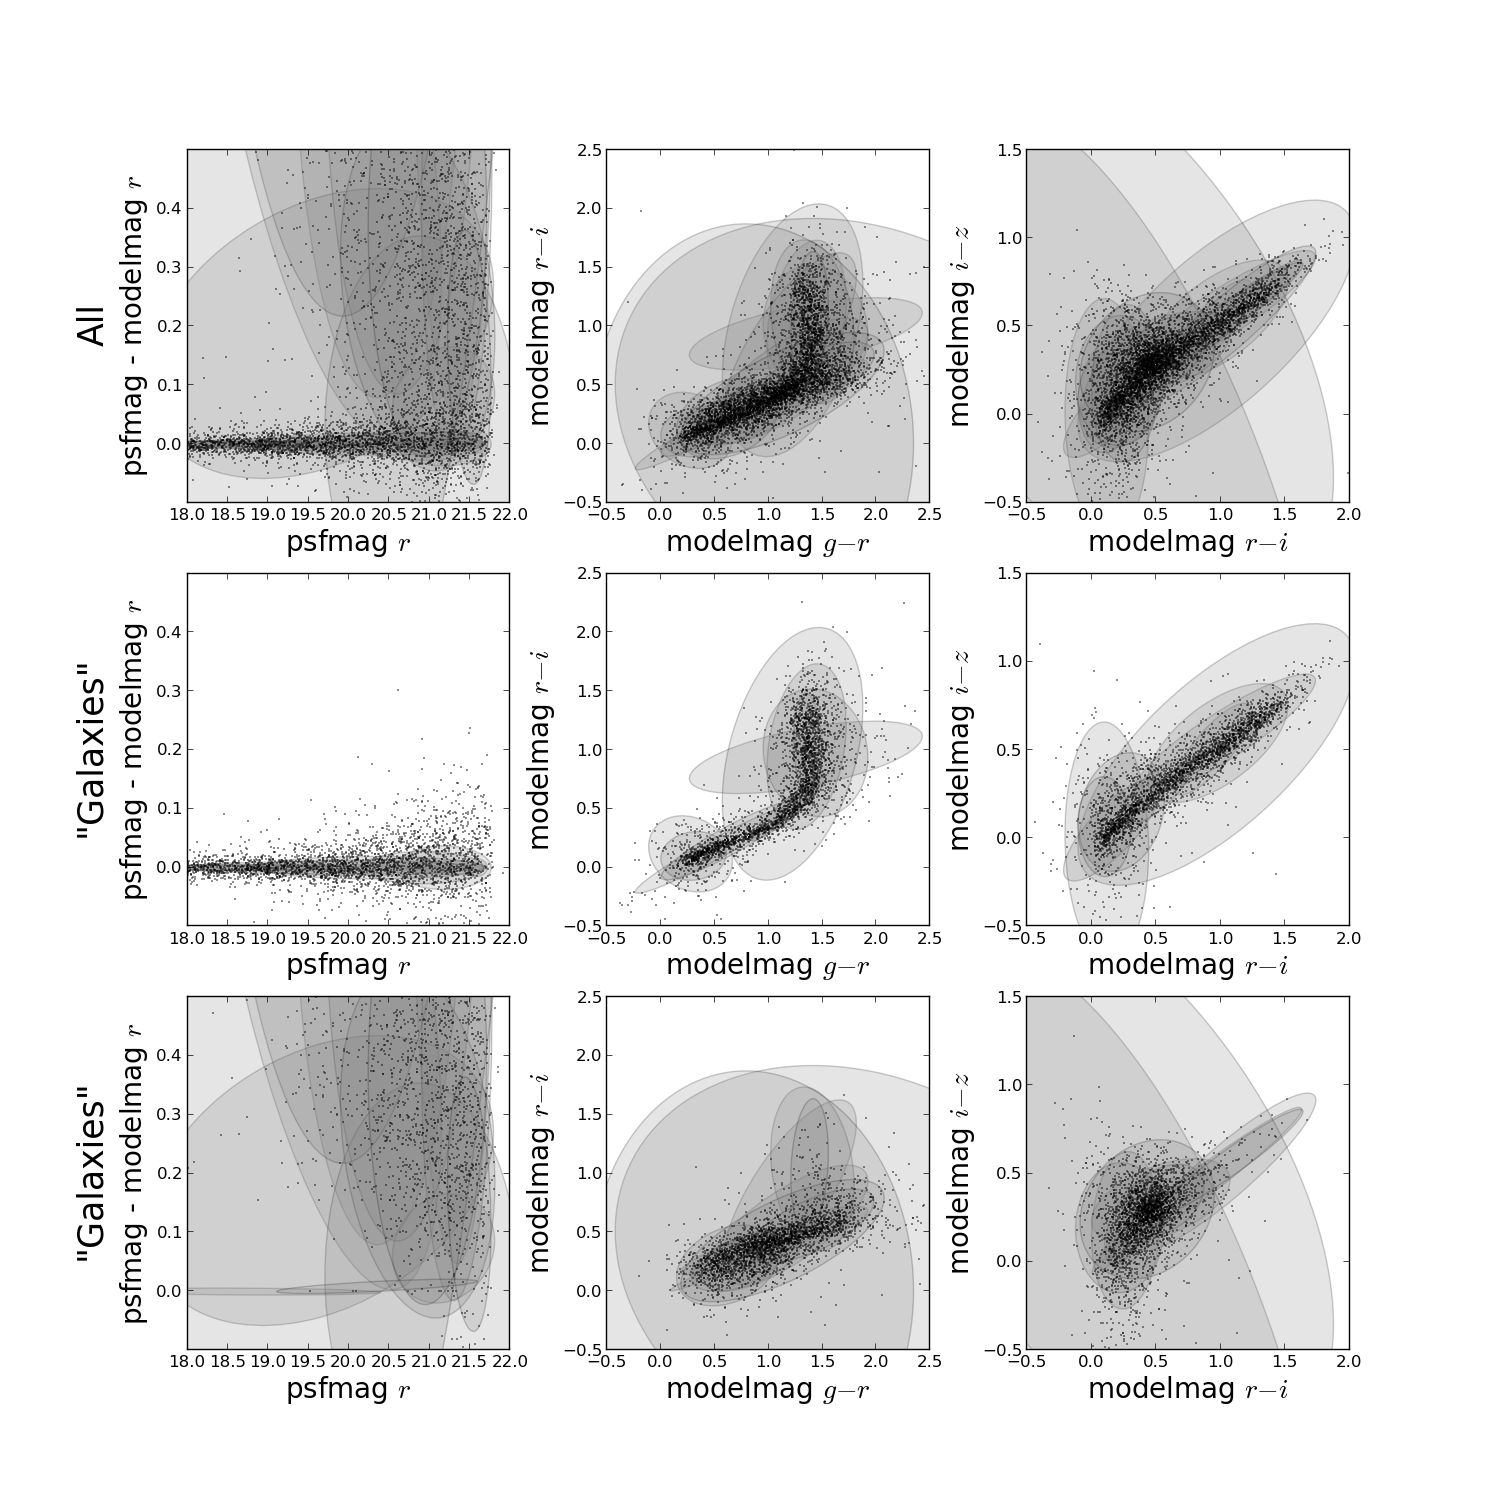
\includegraphics[clip=true, trim=1.5cm 0.5cm 1.5cm 0.5cm,
  width=16cm]{fig1.png}
\caption{Shown are three different projections of one tenth of the DR10
photometric data used (black points), with the top/bottom row corresponding
objects classified as stars/galaxies (\ttt{type} $=6, 3$).  Gray contours
indicate the different XD components.  For the top we only plot the
$N_{\rm point}$ components while in the bottom we plot the rest.  Note,
however, when we compute our model we do not use SDSS classifications -- all
data is modeled with the combination of both top and bottom contours.  Note
the components modeling psfmag minus modelmag for starlike objects prefer
small variance, and generally the model follows the data well.
}
\label{fig:contours}
\end{figure}

\begin{figure}
\centering
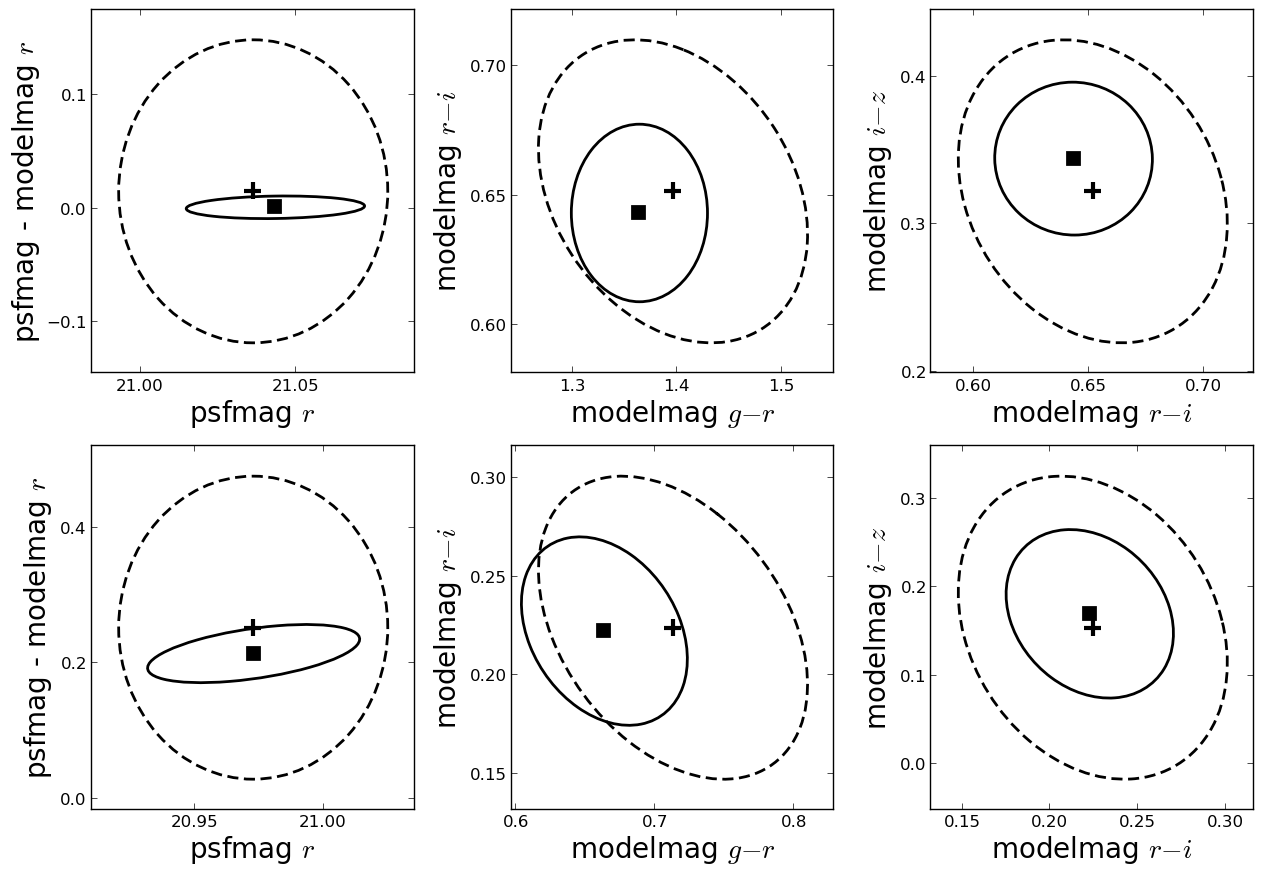
\includegraphics[width=16cm]{fig2.png}
\caption{Error ellipses for single epoch S82 photometry (dashed) and XD
posterior distributions for a star (top row) and galaxy (bottom row).  The 
projections are the same as in Figure \ref{fig:contours}.  Ellipses for the XD
posteriors are generally smaller, yet are still consistent with the original 
measurements.
}
\label{fig:posteriors}
\end{figure}

In figure \ref{fig:posteriors}, we show the posterior distributions for a
random star and galaxy in our sample.  We find generally that projections of 
the posterior are consistent with the original measurements, but are of higher 
precision.  Figure \ref{fig:error_rates} quantifies this, showing the median 
uncertainty as a function of $r$ magnitude.  We find that the median
uncertainties of our XD posteriors are a significant improvement to the
catalog data.  For instance, at $r\sim20$, the uncertainty in the DR10 $r$ PSF 
magnitude is reduced from 0.28 to 0.2 \rf{DOUBLE CHECK} and more dramatically
the error in the $u-g$ model color is reduced from 0.5 to 0.3.  It is not
surprising that the improvements are most significant where the data is more 
noisy since this is where an informative prior can make the most difference.

\begin{figure}
\centering
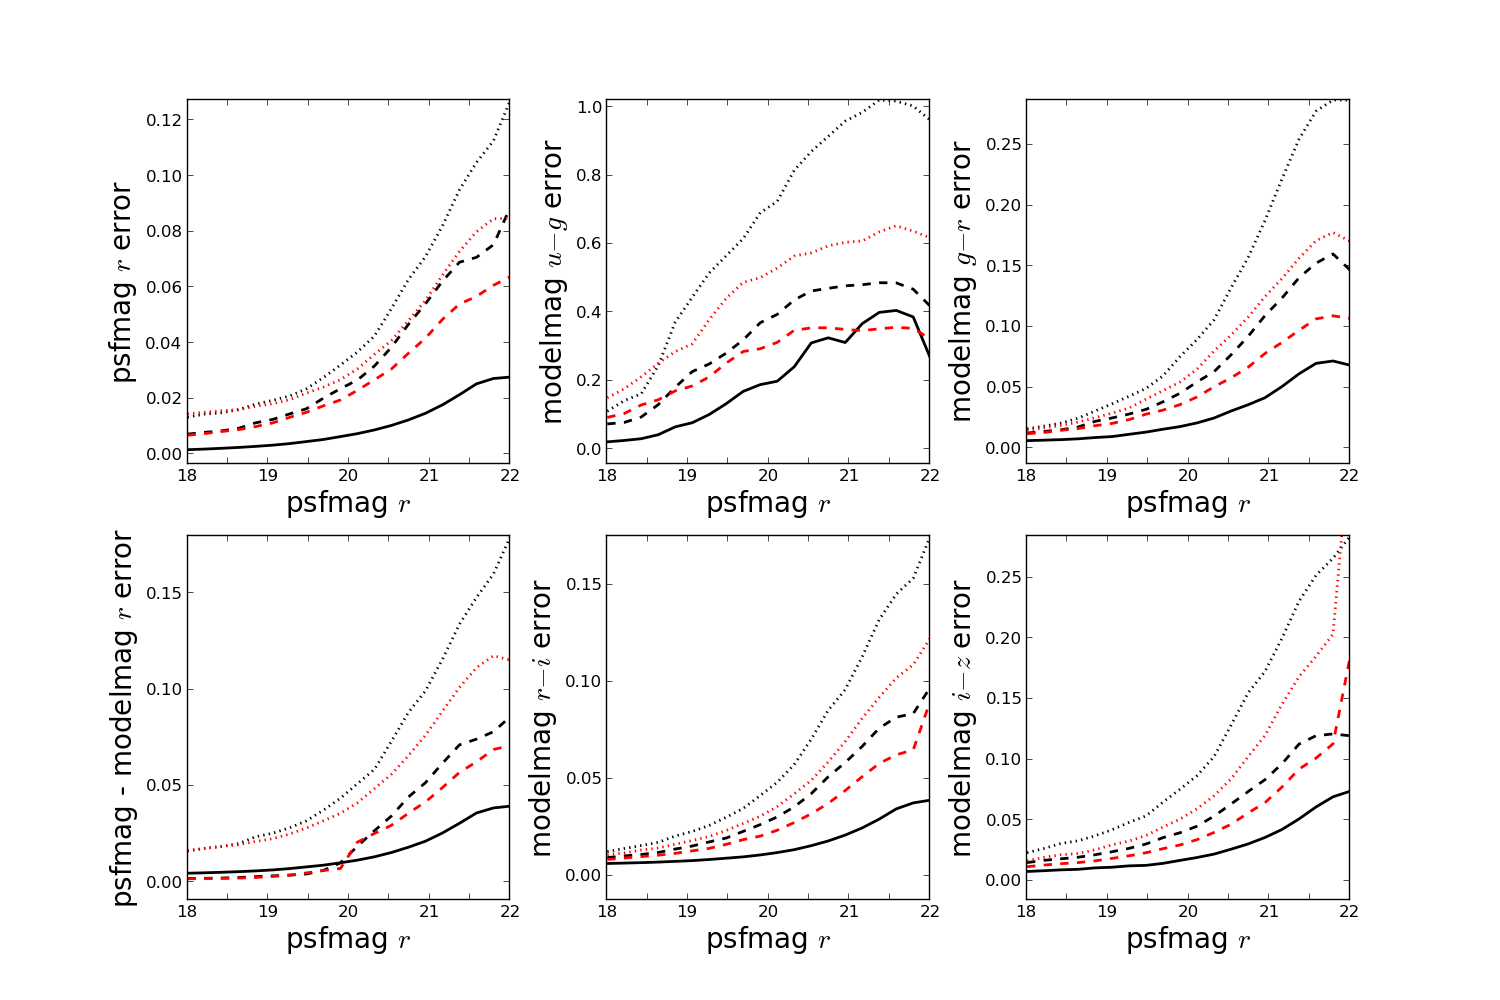
\includegraphics[width=16cm]{fig3.png}
\caption{Plotted are median values for the 1 sigma uncertainty in $r$ PSF
magnitude, $r$
psf minus model magnitude, and the four model colors used.  The solid black 
curve is for the Stripe 82 coadd, while the dotted black and red curves are for
single epoch Stripe 82 and DR10 data, respectively.  The dashed curves show the
median uncertainty for the XD posteriors.  While not quite as precise as the 
coadd data, the XD posteriors are a significant improvement over the catalog
data.
}
\label{fig:error_rates}
\end{figure}

So far we have shown operationally that the XD model does sensible modeling of
the photometry and is more \emph{precise}, but it is important to ask whether
the posteriors are at all \emph{accurate}.  To do so, we rely on comparsions of
the posteriors we get for S82 single epoch data versus the data from the
coadd.  In figure \ref{fig:xx_plots}, we plot the single
epoch data against coadd measurements, as well as our XD posteriors versus the
coadd.  We find that the XD posteriors are in good agreement with the coadd
data -- there is no obvious biases or deviations appart from scatter due to
noise.  We note that there is a slight offset to lower values of $r$ PSF
magnitudes at the faintest end ($r \gtrsim 21.5$).  This is an artifact due to
the fact that none of the components we used were constrained to have mean
around or greater than $r \sim 21.5$.  As a result, the posteriors will
naturally pull the magnitude values down.  A simple fix is to force a few
components of the XD mixture to have means at faint magnitude values, but given
the size of this effect we have not done so for the purposes here.  Note a
similar effect will also occur at the bright end of our sample, but is less 
significant since the measurement uncertainties are lower.  As a additional 
demonstration of the reasonability of our method, we show the color-magnitude
diagram for DR10 data of the globular cluster Messier 3 in Figure
\ref{fig:m3}.  Compared to the DR10 data the XD posterior is clearly much
cleaner at faint $r$ magnitudes, and is more concentrated across much of the
main sequence.  Note that the width of the main sequence around $r \sim 19$ is
not dramatically changed from DR10.  This is because the measurement
uncertainties are fairly small so the DR10 value is the dominant contributor
to the posterior.  In other words, the XD values seem to be respectful of the 
data and do not seem to overly `denoise'.

\begin{figure}
\centering
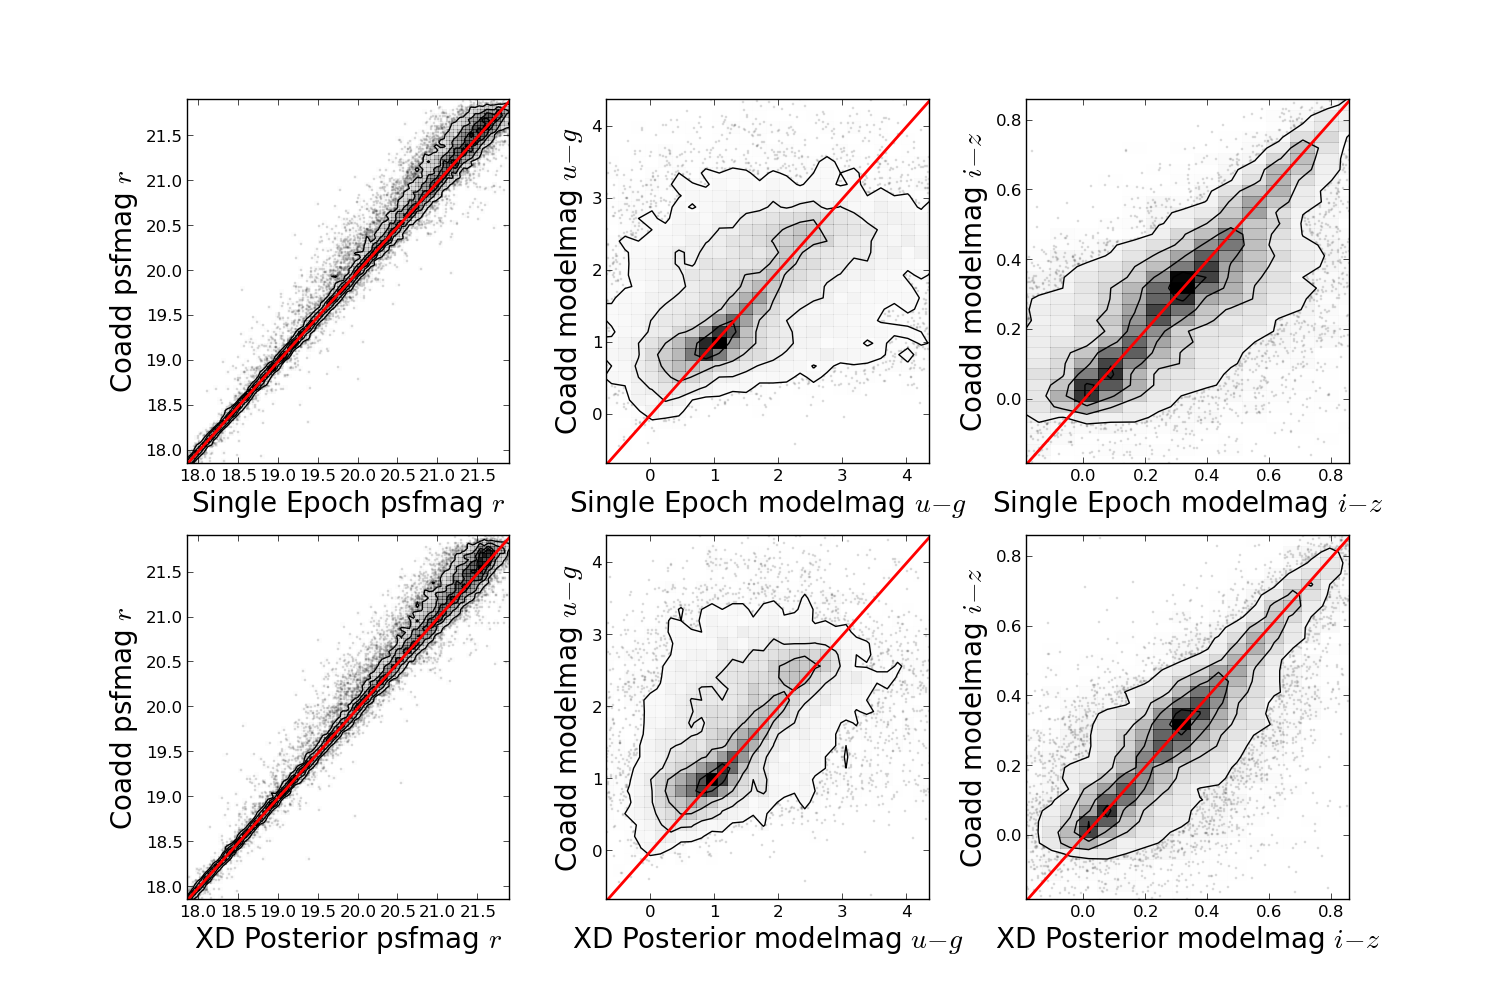
\includegraphics[width=16cm]{fig4.png}
\caption{In the top row, we plot 2D histograms of $r$ PSF magnitudes, $u-g$
model color, and $i-z$ model color for single epoch Stripe 82 data versus the
corresponding coadd values.  In the bottow row, we plot the same for a single
sample from the XD posteriors of the data in the top.  Generally speaking the
XD posteriors are very consistent with the coadd photometry, indicating that 
the models are indeed acurate.
}
\label{fig:xx_plots}
\end{figure}

\begin{figure}
\centering
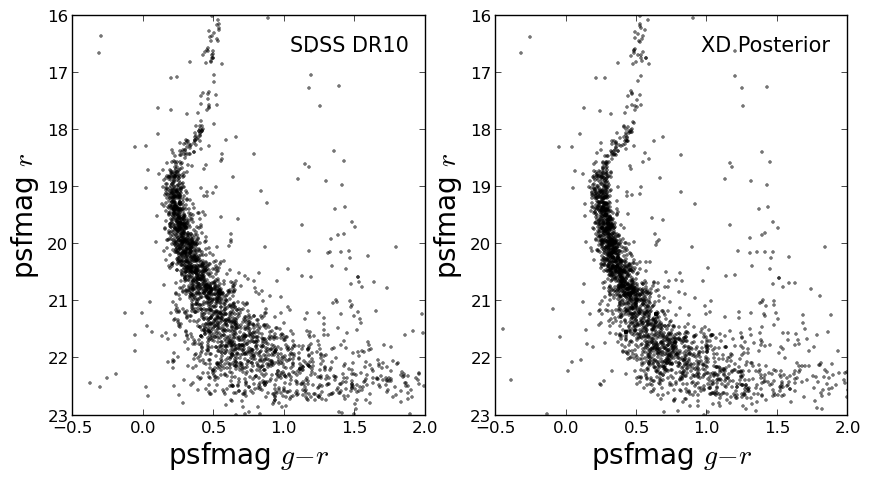
\includegraphics[width=16cm]{fig5.png}
\caption{The $g-r$ versus $r$ color-magnitude diagram from the outskirts of
the globular cluster Messier 3.  The left panel shows the original DR10
measurements and the right shows the median value from the XD posteriors.  Note
the main sequence is generally more concentrated, especially at faint
magnitudes.
}
\label{fig:m3}
\end{figure}

In SDSS, star-galaxy classification is accomplished by selecting objects a
small range of PSF minus model magnitudes and calling them stars.  In DR10,
the range is approximately\footnote{The actual algorithm involves a combination
of this criterion for $gri$ bands.} $|r_{PSF} - r_{model}| < 0.145$ while the
S82 coadd criterion is $|r_{PSF} - r_{model}| < 0.03$.  In figure \ref{fig:pmm}
we show a histogram of $r$ PSF minus model magnitudes around $r=19.5$
20.5, and 21.5 for objects that are called `stars' in the coadd.  Note that
our XD posteriors dramatically tighten the distribution of objects to values
very close to zero.  This implies that the quality of the star-galaxy
classification could be substantially improved by selecting on values produced
by the XD posteriors.

\begin{figure}
\centering
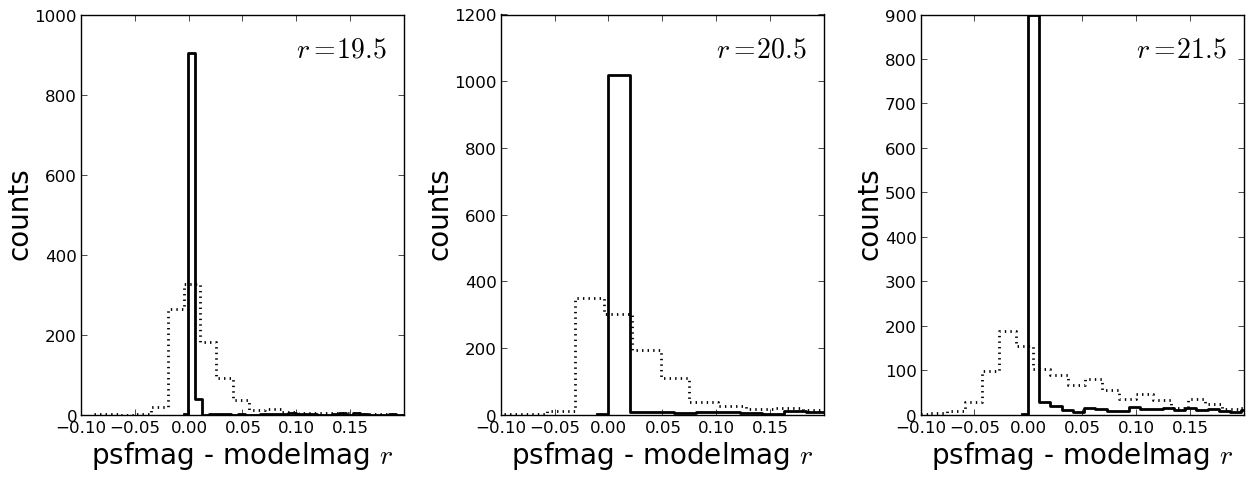
\includegraphics[width=16cm]{fig6.png}
\caption{Histograms of the values of the $r$ PSF minus model magnitudes for 
objects within 0.15 mag of $r = 19.5$, 20.5, and 21.5 that were labeled as 
`stars' in the Stripe 82 coadd.  The dotted histograms shows the distribution
for single epoch Stripe 82 data, while the solid histograms show those for the
XD posteriors.  The XD values are strongly peaked near zero, while the single
epoch values are more distributed, suggesting star-galaxy classification
could be improved by relying on the XD values.  
}
\label{fig:pmm}
\end{figure}

We emphasize that the method we present here is just a toy example of how one 
might improve photometric measurements in astronomical surveys.  By no means do
we believe that this is the best or only way to build a hierarchical model for 
the photometry, however, it does have the property of being simple,
interpretable, and yet quite flexible.  For a ``production'' level set of
posteriors there would still be much to sort out, including ---

\begin{itemize}
\item What data should be used for training the XD model?
\item What are the optimal number of XD components?
\item Which mean values of the mixture should be fixed
\item Which covariances should be diagonal?
\item What are the best features to include model?
\item What, if any, features should be included that are outside the survey
data?
\end{itemize}

All such questions would be straightforward to answer using cross validation,
either on left out ``test'' data or higher signal-to-noise data.  One of the
main reasons that we have not done so here is that the correct metric for any
cross validation approach depends on the scientific goals of the experiment.  
Large surveys can likely define a set of such metrics that meet much of their 
users goals, but there may still be cases where individuals may want to define
their own models.  Finally, we do not argue that posterior values should 
replace photometric measurements in all cases.  Indeed, in the case transient
or varying objects this would likely be a bad idea.  Additionally, it may
hinder the discovery of rare types of objects since the prior would drive the
measurments to values like more common sources.

\end{document}
